\subsection{Sprint 1: da 2024-04-03 a 2024-04-19}
\par In seguito all'aggiudicazione dell'appalto, il team ha optato per una finestra temporale di oltre due settimane da dedicare al primo periodo. Questa decisione è motivata dal fatto che le fasi preliminari del progetto richiedono uno studio e una sperimentazione delle mansioni che ciascun componente sarà chiamato a ricoprire. Inoltre, la concomitanza con i colloqui per lo stage potrebbe ridurre significativamente le ore produttive giornaliere. Nell'arco del primo \glossario{sprint}, il team si focalizzerà sulla configurazione dell'ambiente di lavoro (con annessa definizione dei processi di automazione), sulla stesura della documentazione di progetto e sull'\AdR.

\subsubsection{Obiettivi}
\begin{itemize}
  \item Aggiornamento del template \glossario{LaTeX} per l'elaborazione dei documenti;
  \item Miglioramento continuo del \glossario{\WoW};
  \item Stesura del documento \NdP, al cui interno saranno formalizzate le procedure, le linee guida e gli strumenti a supporto del lavoro di gruppo;
  \item Raccolta dei termini da inserire nel \Gls;
  \item Scelta del modello di sviluppo;
  \item Creazione di una dashboard su \glossario{Google Sheets} per realizzare preventivo e consuntivo degli \glossario{sprint}, rendicontare le ore e generare grafici in tempo reale;
  \item Redazione del documento di \AdR, con un focus sugli \glossario{attori} che interagiscono con il sistema e sul modo in cui vi interagiscono;
  \item Definizione dei primi \glossario{casi d'uso} da discutere con la \glossario{Proponente};
  \item Creazione del \glossario{repository} ChatSQL su \glossario{GitHub} per il \glossario{versionamento} del codice sorgente;
  \item Definizione iniziale del \glossario{dizionario dati};
  \item Stesura verbali interni ed esterni.
\end{itemize}

\begin{figure}[H]
  \centering
  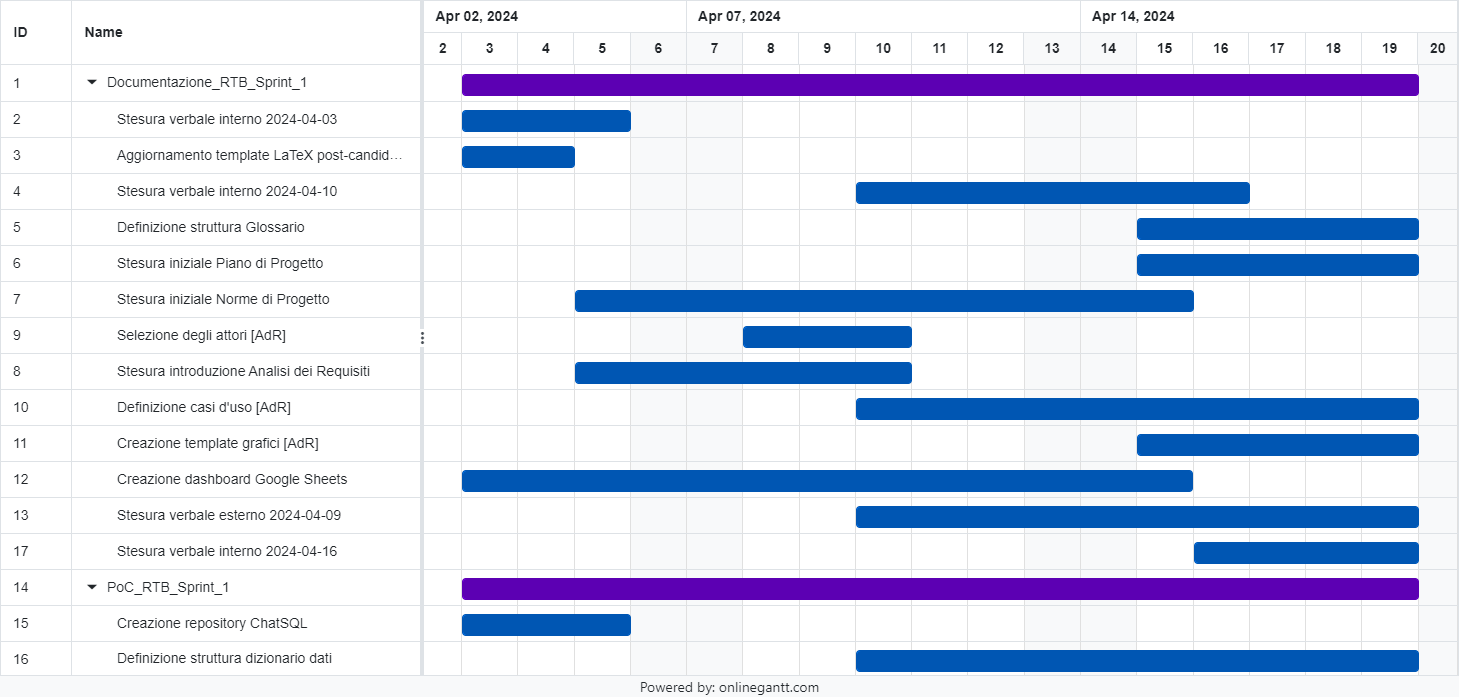
\includegraphics[width=0.90\textwidth]{assets/Pianificazione/Sprint-1/gantt.png}
  \caption{Sprint 1 - Diagramma di Gantt}\label{fig:sprint-1-gantt}
\end{figure}
 